\documentclass[journal,12pt,twocolumn]{IEEEtran}
%
\makeatletter
\makeatother
\usepackage{setspace}
\usepackage{gensymb}
\usepackage{xcolor}
\usepackage{caption}
%\usepackage{stackengine}
%\usepackage{subcaption}
%\doublespacing
\singlespacing



\usepackage{graphicx}
\graphicspath{ {./images}  }
%\usepackage{amssymb}
%\usepackage{relsize}
\usepackage[cmex10]{amsmath}
\usepackage{mathtools}
%\usepackage{amsthm}
%\interdisplaylinepenalty=2500
%\savesymbol{iint}
%\usepackage{txfonts}
%\restoresymbol{TXF}{iint}
\usepackage{wasysym}
\usepackage{amsthm}
\usepackage{mathrsfs}
\usepackage{txfonts}
\usepackage{stfloats}
\usepackage{cite}
\usepackage{cases}
\usepackage{mathtools}
\usepackage{subfig}
\usepackage{enumerate}	
\usepackage{enumitem}
\usepackage{amsmath}
%\usepackage{xtab}
\usepackage{longtable}
\usepackage{multirow}
%\usepackage{algorithm}
%\usepackage{algpseudocode}
\usepackage{enumitem}
\usepackage{mathtools}
%\usepackage{iithtlc}
%\usepackage[framemethod=tikz]{mdframed}
\usepackage{listings}
\usepackage{listings}
    \usepackage[latin1]{inputenc}                                 %%
    \usepackage{color}                                            %%
    \usepackage{array}                                            %%
    \usepackage{longtable}                                        %%
    \usepackage{calc}                                             %%
    \usepackage{multirow}                                         %%
    \usepackage{hhline}                                           %%
    \usepackage{ifthen}                                           %%
  %optionally (for landscape tables embedded in another document): %%
    \usepackage{lscape}     



%\usepackage{stmaryrd}


%\usepackage{wasysym}
%\newcounter{MYtempeqncnt}
\DeclareMathOperator*{\Res}{Res}
%\renewcommand{\baselinestretch}{4}
%\setcounter{secnumdepth}{4}
\renewcommand\thesection{\arabic{section}}
\renewcommand\thesubsection{\thesection.\arabic{subsection}}
\renewcommand\thesubsubsection{\thesubsection.\arabic{subsubsection}}
%\renewcommand\thesubsubsubsection{\thesubsubsection.\arabic{subsubsubsection}}

%\renewcommand\thesectiondis{\arabic{section}}
%\renewcommand\thesubsectiondis{\thesectiondis.\arabic{subsection}}
%\renewcommand\thesubsubsectiondis{\thesubsectiondis.\arabic{subsubsection}}
%\renewcommand\thesubsubsubsectiondis{\thesubsubsectiondis.\arabic{subsubsubsection}}
% correct bad hyphenation here
\hyphenation{op-tical net-works semi-conduc-tor}

%\lstset{
%language=C,
%frame=single, 
%breaklines=true
%}

%\lstset{
	%%basicstyle=\small\ttfamily\bfseries,
	%%numberstyle=\small\ttfamily,
	%language=Octave,
	%backgroundcolor=\color{white},
	%%frame=single,
	%%keywordstyle=\bfseries,
	%%breaklines=true,
	%%showstringspaces=false,
	%%xleftmargin=-10mm,
	%%aboveskip=-1mm,
	%%belowskip=0mm
%}

%\surroundwithmdframed[width=\columnwidth]{lstlisting}
\def\inputGnumericTable{}                                 %%

\lstset{
%language=python,
frame=single, 
breaklines=true,
columns=fullflexible
}

 

\begin{document}
%

\theoremstyle{definition}
\newtheorem{theorem}{Theorem}[section]
\newtheorem{problem}{Problem}
\newtheorem{proposition}{Proposition}[section]
\newtheorem{lemma}{Lemma}[section]
\newtheorem{corollary}[theorem]{Corollary}
\newtheorem{example}{Example}[section]
\newtheorem{definition}{Definition}[section]
%\newtheorem{algorithm}{Algorithm}[section]
%\newtheorem{cor}{Corollary}
\newcommand{\BEQA}{\begin{eqnarray}}
\newcommand{\EEQA}{\end{eqnarray}}
\newcommand{\define}{\stackrel{\triangle}{=}}
\bibliographystyle{IEEEtran}
%\bibliographystyle{ieeetr}
\providecommand{\nCr}[2]{\,^{#1}C_{#2}} % nCr
\providecommand{\nPr}[2]{\,^{#1}P_{#2}} % nPr
\providecommand{\mbf}{\mathbf}
\providecommand{\pr}[1]{\ensuremath{\Pr\left(#1\right)}}
\providecommand{\qfunc}[1]{\ensuremath{Q\left(#1\right)}}
\providecommand{\sbrak}[1]{\ensuremath{{}\left[#1\right]}}
\providecommand{\lsbrak}[1]{\ensuremath{{}\left[#1\right.}}
\providecommand{\rsbrak}[1]{\ensuremath{{}\left.#1\right]}}
\providecommand{\brak}[1]{\ensuremath{\left(#1\right)}}
\providecommand{\lbrak}[1]{\ensuremath{\left(#1\right.}}
\providecommand{\rbrak}[1]{\ensuremath{\left.#1\right)}}
\providecommand{\cbrak}[1]{\ensuremath{\left\{#1\right\}}}
\providecommand{\lcbrak}[1]{\ensuremath{\left\{#1\right.}}
\providecommand{\rcbrak}[1]{\ensuremath{\left.#1\right\}}}
\theoremstyle{remark}
\newtheorem{rem}{Remark}
\newcommand{\sgn}{\mathop{\mathrm{sgn}}}
\providecommand{\abs}[1]{\left\vert#1\right\vert}
\providecommand{\res}[1]{\Res\displaylimits_{#1}} 
\providecommand{\norm}[1]{\lVert#1\rVert}
\providecommand{\mtx}[1]{\mathbf{#1}}
\providecommand{\mean}[1]{E\left[ #1 \right]}
\providecommand{\fourier}{\overset{\mathcal{F}}{ \rightleftharpoons}}
%\providecommand{\hilbert}{\overset{\mathcal{H}}{ \rightleftharpoons}}
\providecommand{\system}{\overset{\mathcal{H}}{ \longleftrightarrow}}
	%\newcommand{\solution}[2]{\textbf{Solution:}{#1}}
\newcommand{\solution}{\noindent \textbf{Solution: }}
\providecommand{\dec}[2]{\ensuremath{\overset{#1}{\underset{#2}{\gtrless}}}}
\DeclarePairedDelimiter{\ceil}{\lceil}{\rceil}
%\numberwithin{equation}{subsection}
\numberwithin{equation}{section}
%\numberwithin{problem}{subsection}
%\numberwithin{definition}{subsection}
%\makeatletter
%\@addtoreset{figure}{section}
%\makeatother
\let\StandardTheFigure\thefigure
%\renewcommand{\thefigure}{\theproblem.\arabic{figure}}
%\renewcommand{\thefigure}{\thesection}
%\numberwithin{figure}{subsection}
%\numberwithin{equation}{subsection}
%\numberwithin{equation}{section}
%\numberwithin{equation}{problem}
%\numberwithin{problem}{subsection}
%\numberwithin{problem}{section}
%%\numberwithin{definition}{subsection}
%\makeatletter
%\@addtoreset{figure}{problem}
%\makeatother
%\makeatletter
%\@addtoreset{table}{problem}
%\makeatother
\let\StandardTheFigure\thefigure
\let\StandardTheTable\thetable
%%\renewcommand{\thefigure}{\theproblem.\arabic{figure}}
%\renewcommand{\thefigure}{\theproblem}
%%\numberwithin{figure}{section}
%%\numberwithin{figure}{subsection}
\def\putbox#1#2#3{\makebox[0in][l]{\makebox[#1][l]{}\raisebox{\baselineskip}[0in][0in]{\raisebox{#2}[0in][0in]{#3}}}}
     \def\rightbox#1{\makebox[0in][r]{#1}}
     \def\centbox#1{\makebox[0in]{#1}}
     \def\topbox#1{\raisebox{-\baselineskip}[0in][0in]{#1}}
     \def\midbox#1{\raisebox{-0.5\baselineskip}[0in][0in]{#1}}
\title{ 
%	\logo{
Frame Synchronization : Global Summation of SOF/PLSC Detectors%	}
}
\author{Theresh Babu Benguluri, Raktim Goswami, Abhishek Bairagi, Siddharth Maurya, Pappu Manasa, Sandeep Khyalia  , Raja Pradyumna , B Swaroop reddy and G V V 
Sharma$^{*}$% <-this % stops a space
\thanks{*The authors are with the Department
of Electrical Engineering, Indian Institute of Technology, Hyderabad
502285 India e-mail:  gadepall@iith.ac.in.}
}
% make the title area
\maketitle
%\tableofcontents
\bigskip
%
\begin{abstract}
%\boldmath
This manual provides a brief description about the design and implementation of digital 
synchronization techniques for reliable communication.
\end{abstract}
%\IEEEpeerreviewmaketitle
%
\section{Frame Synchronization : Global Summation of SOF/PLSC Detectors} 
%
%
Let the frequency offset be $\Delta f$ and phase offset be $\Delta \phi$.Then,
\begin{equation}
%\label{eq:freq_offset_model}
Y_k= X_k e^{j(2\pi\Delta fkM+\phi_k)} + V_k, \quad k = 1,\dots,N 
\end{equation}
%
assuming that no pilot symbols are trasmitted. 
Let the phase information be $\theta_k$, and defined as
%
\begin{equation}
e^{\theta(k)} = \frac{Y_k}{\abs{Y_k}}
\end{equation}
%
At the receiver, the header information is available in the form of 
\begin{align}
g_i(l)&=x_s(l)x_s(l-i), l = 0,\dots, SOF-1
\\
h_i(l)&=x_p(l)x_p(l-i), l = 0,\dots, PLSC-1
\end{align}
%
where $x_s$ are the mapped SOF symbols, $x_p$ are the scrambled PLSC  symbols, both  modulated using 8-PSK
for $i=1,2,4,8,16,32$.
The SOM is choosen as a 64-bit length such that SOF and PLS each are of 32-bit length.

A special kind of correlation is performed to obtain
\begin{align}
m_i(k)&=\sum_{l=0}^{PLSC-1} e^{j(\theta(k-l)-\theta(k-l-i))} h_i(l),
\\
n_i(k)&=\sum_{l=0}^{SOF-1} e^{j(\theta(k-l)-\theta(k-l-i))} g_i(l) ,
\\
&k = 1, \dots, N 
\end{align}
%
Compute
\begin{align}
p_i(k)=
\begin{cases}
\max \lbrak{\abs{n_i({k-PLSC})+m_i(k)},} &
\\
\rbrak{\abs{n_i({k-PLSC})-m_i(k)}} & k > PLSC
%\max \abs{m_i(k)}  & k < 64
\end{cases}
\end{align}
 GLOBAL variable $G_{R,T}(k)$  \cite{frame_offset} defined as,
\begin{equation}
G_{R,T}(k)=\sum_{i\geq1}p_i(k) , \quad i=1,2,4,8,16,32
\label{eq:global}
\end{equation}
At the receiver, let us consider we have sent two types of transmission. One is PLHEADER+DATA $\brak{Y_{k1}}$ and another is only DATA $\brak{Y_{k2}}$ and the GLOBAL variables for $\brak{Y_{k1}}$ and $\brak{Y_{k2}}$ from \eqref{eq:global} are $G1_{R,T}(k)$, $G2_{R,T}(k)$ respectively.
\subsection{Global Threshold Calculation}
The Global Threshold variable is defined as
\begin{align}
T&= \max \brak{ \max \brak{G1_{R,T}(k)},\max \brak{ G2_{R,T}(k)}}
\end{align} 
%\subsection{False Alarm Probability}
The probability of false detection of plheader when only DATA frame $\brak{Y_{k2}}$ has been sent is defined as
\begin{align}
P_{FA} &= \frac{\sum \frac{sign(\abs{Y_{k2}-T})+1}{2} }{N}
\end{align}
%\subsection{Missed Detection Probability}
The probability of missed detection of plheader when PLHEADER+DATA $\brak{Y_{k1}}$ has been sent is defined as
\begin{align}
P_{MD} &= \frac{\sum \frac{sign(T-\abs{Y_{k1}})+1}{2} }{N+PLSC+SOF}
\end{align}
%\subsection{False Alarm Probability}
%False Alarm Probability $(p_{fa})$, is the probability of false detection of plheader when only DATA frame has been sent.
%%\subsection{Missed Detection Probability}
%Missed Detection Probabililty $(p_{md})$, is the probability of missed detection of plheader when PLHEADER+DATA has been sent.
\subsection{Plots}
\begin{figure}[!t]
\begin{center}
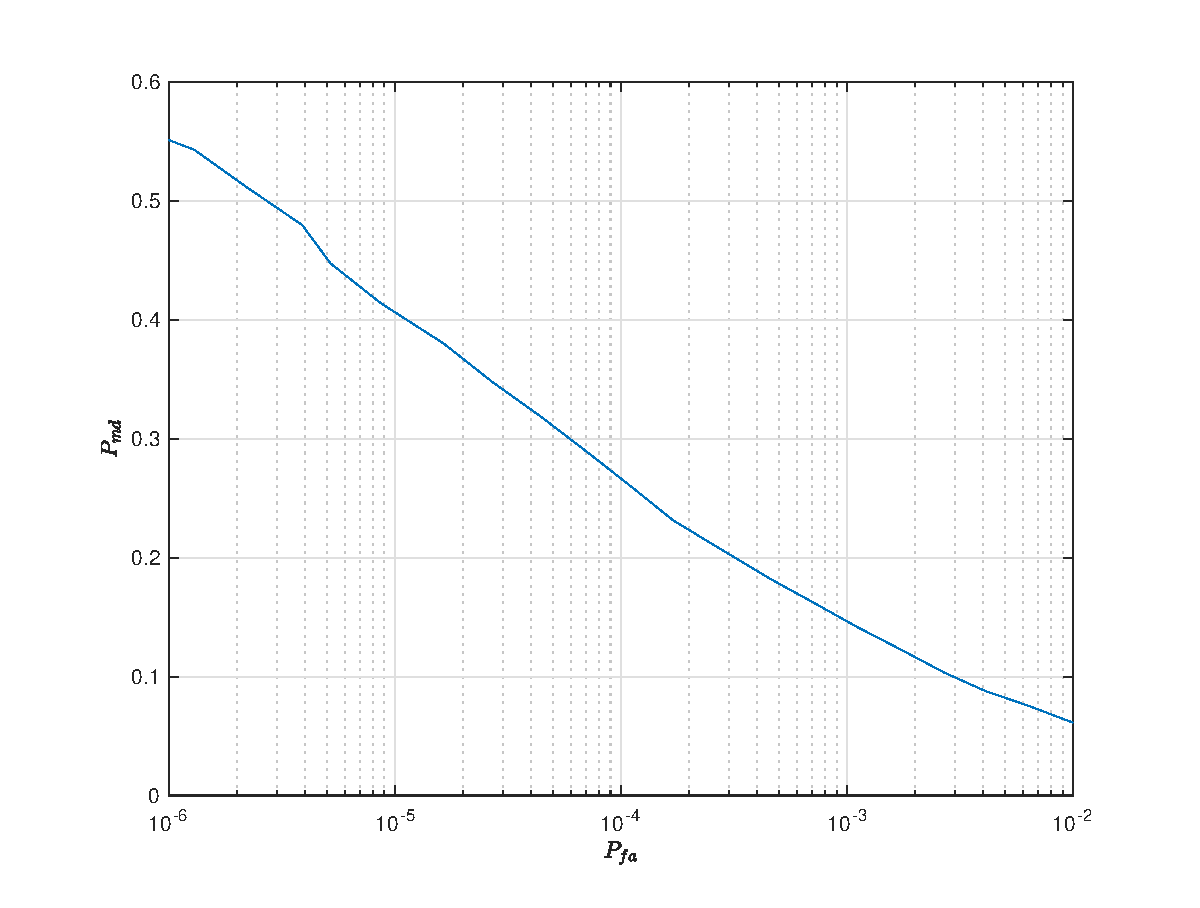
\includegraphics[width=\columnwidth]{../figs/ROC.eps}
\end{center}
\caption{Frame Synchronization Receiver Operating Characteristcs (ROC)}
\label{fig:frameoff}
\end{figure}
Fig.\ref{fig:frameoff} shows the ROC curve ($P_{FA} vs P_{MD}$)  at the receiver for frame synchronization at $\frac{E_b}{N_0}=-2$ dB and with a frequency offset of 250 KHz.
%
\bibliography{IEEEabrv,frame_detection.bib}
%\begin{thebibliography}{20}
%\bibitem{1}
%U. Mengali and A. N. D'Andrea:'synchronization Techniques for Digital Receivers,' New York: Plenum, 1997.
%
%\bibitem{2}
%F. M. Gardner:'A BPSK/QPSK timing-error detector for sampled receivers,' IEEE TRANSACTIONS ON COMMUNICATIONS, VOL.COM-34,NO.5,MAY 1986
%\bibitem{3}
%M. Luise and R. Reggiannini:'Carrier frequency recovery in all-digital modems for burst mode transmissions,' IEEE Trans. Commun., vol. 43,
%no. 2/3/4, pp. 1169-1178, Feb/Mar/Apr 1995.
%
%\bibitem{4}
%E. Casini, R. De Gaudenzi, and A. Ginesi:'DVB-S2 modem algorithms
%design and performance over typical satellite channels,' International
%Journal of Satellite Communications and Networking 2004, vol. 22(3), pp. 281-318, 2004.
%
%
%\end{thebibliography}
\end{document}
